\documentclass{article}

\usepackage[margin=1in]{geometry}
\usepackage{graphicx}
\usepackage{pgfgantt}
\usepackage{xcolor}

\title{The Gentrification of the San Francisco Bay Area \\ \large TEAM-17 Progress Report}
\author{Benicio Bailey, Jacob Feenstra, Diane Kim, Aryan Sarda}

\begin{document}
\maketitle

\section{Method}

\begin{itemize}
\item  Provide a detailed explanation of your current design (nearly done) and implementation (at least half done), covering both the visualization and storytelling aspects.
\item  List any significant changes, design decisions, or improvements made since the proposal. Include figures or diagrams if they help clarify your method.
\end{itemize}

\graphicspath{{../imgs/}}

\begin{figure}[h!]
    \centering
    \begin{minipage}{0.48\textwidth}
        \centering
        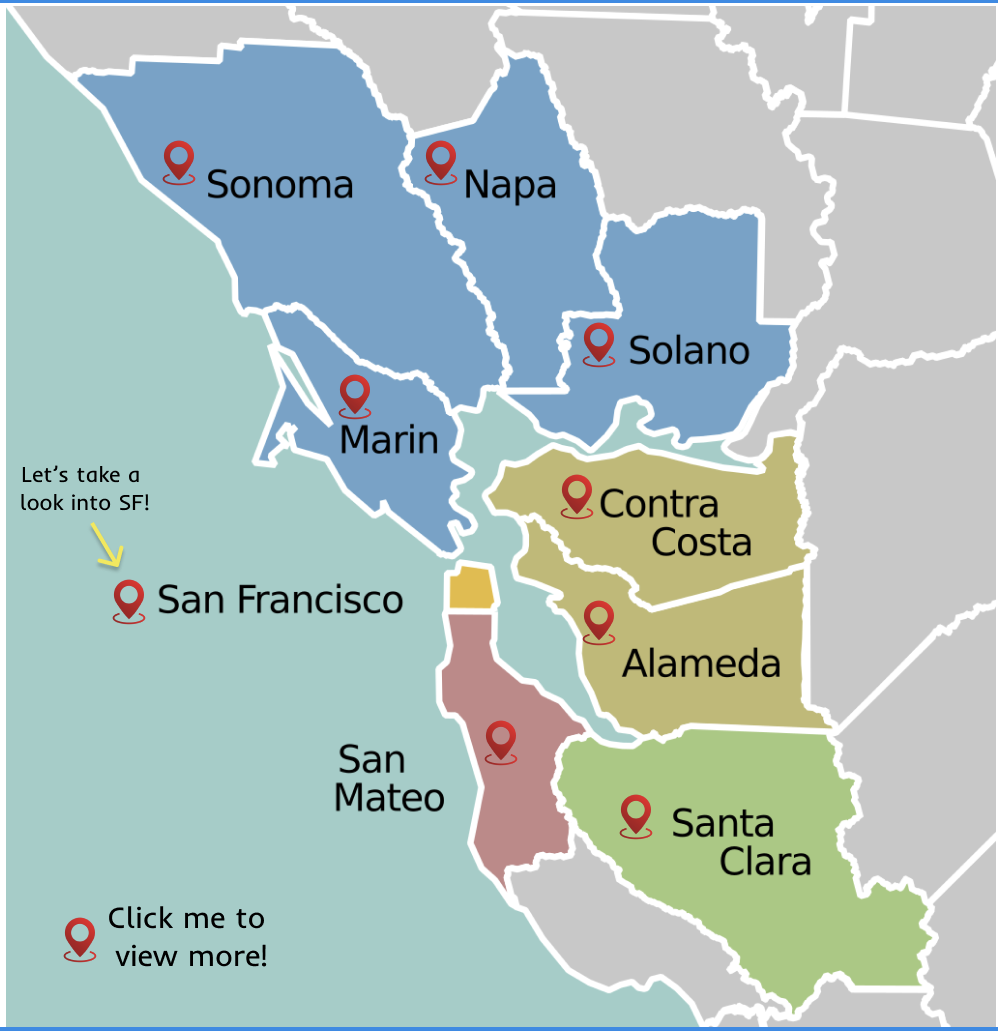
\includegraphics[width=\linewidth]{fig1.png}
        \caption{View of the Bay Area}
        \label{fig:first}
    \end{minipage}\hfill 
    \begin{minipage}{0.48\textwidth}
        \centering
        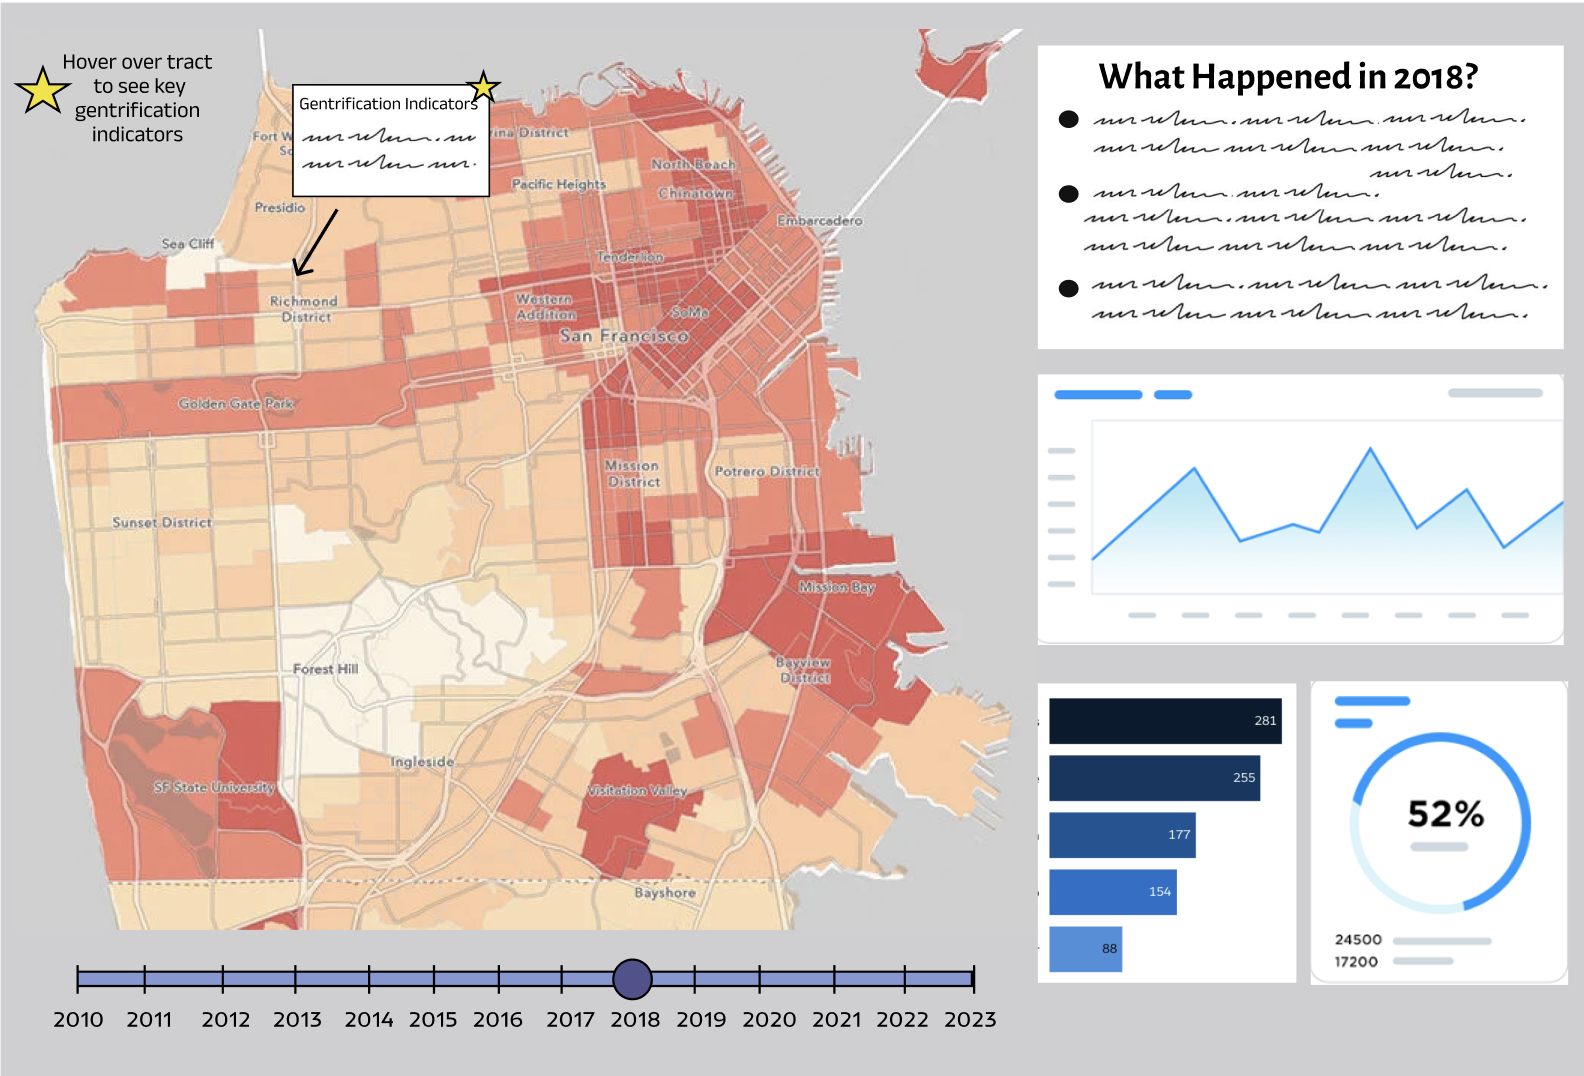
\includegraphics[width=\linewidth]{fig2.png}
        \caption{View of San Francisco County, by census tract}
        \label{fig:second}
    \end{minipage}
    \caption{Drill-Down approach to explore Bay Area counties}
    \label{fig:combined}
\end{figure}

\begin{enumerate}
\item Yep, this is happening.
\item and so is this!
\end{enumerate}

\section{Evaluation Plan}

\begin{itemize}
\item  Describe how you plan to evaluate your system. 
\end{itemize}


\section{Preliminary Results}

\begin{itemize}
\item  Report any results/insights obtained so far. If no results are yet available, describe what results/insights you expect to generate and how they would support your claims.
\end{itemize}

\section{Plan of Activities}

\begin{itemize}
\item  Present your latest activity plan, using either a Gantt chart (example) or a table. For each task, include: (a) Who is responsible, (b) The start and end time (or duration), and (c) Whether the task is complete, ongoing, or upcoming. 
\end{itemize}

% making a gantt chart
The following Gantt chart illustrates the timeline of key project tasks:

\begin{center}
\begin{ganttchart}[
  hgrid,
  vgrid,
  time slot format=isodate,
  time slot unit=day,
  x unit=0.7cm,
  y unit chart=0.8cm,
  title/.style={draw=none, fill=gray!20},
  title label font=\bfseries\footnotesize,
  bar/.style={fill=blue!50},
  bar label font=\small\color{black},
  bar label node/.append style={align=center, text width=4.5cm},
  bar height=0.6,
]{2025-05-21}{2025-06-05}

\gantttitle{Project Timeline}{16} \\
\gantttitlecalendar{month=name, day=2} \\

\ganttbar[
  progress=100
]{data preprocessing\\(Jacob)}{2025-05-21}{2025-05-23} \\

\ganttbar[
  progress=100
]{progress report\\(Jacob)}{2025-05-23}{2025-05-26} \\

\ganttbar[
  progress=0
]{video presentations\\(all)}{2025-06-02}{2025-06-05} \\

\ganttbar[
  progress=40
]{timeline annotations\\(Jacob)}{2025-05-26}{2025-06-02} \\

\ganttbar[
  progress=50
]{martini glass intro\\(Jacob)}{2025-05-26}{2025-06-01} \\

\ganttbar[
  progress=10
]{bay area map \& interactivity\\(Aryan)}{2025-05-23}{2025-06-02}\\

\ganttbar[
  progress=0
]{json county maps\\{(Benicio)}}{2025-05-23}{2025-05-28} \\

\ganttbar[
  progress=10
]{county vis dashboard\\(Diane)}{2025-05-23}{2025-06-03} \\

\ganttbar[
  progress=20
]{9 census tract heatmaps\\(Benicio)}{2025-05-23}{2025-06-03} \\

\ganttbar[
  progress=10
]{2010-2023 timeline\\(Diane)}{2025-05-23}{2025-06-03} \\

\ganttbar[
  progress=0
]{testing \& review\\(all)}{2025-06-03}{2025-06-04} \\

\ganttbar[
  progress=0
]{final report\\(Jacob)}{2025-06-01}{2025-06-05} \\

\end{ganttchart}
\end{center}


\section{Team's Effort Division}

\begin{itemize}
\item Please provide a brief effort distribution statement at the end. It can be as simple as "all team members have contributed a similar amount of effort". If effort distribution is too uneven, we might consider assigning higher scores to members who have contributed more.
\end{itemize}

\nocite{*}
\bibliographystyle{alpha}
\bibliography{refs}

\end{document}